% !TeX root = Protokoll.tex
\subsection{Amplitudenmodulation}
\begin{figure}[h!]
	\centering
	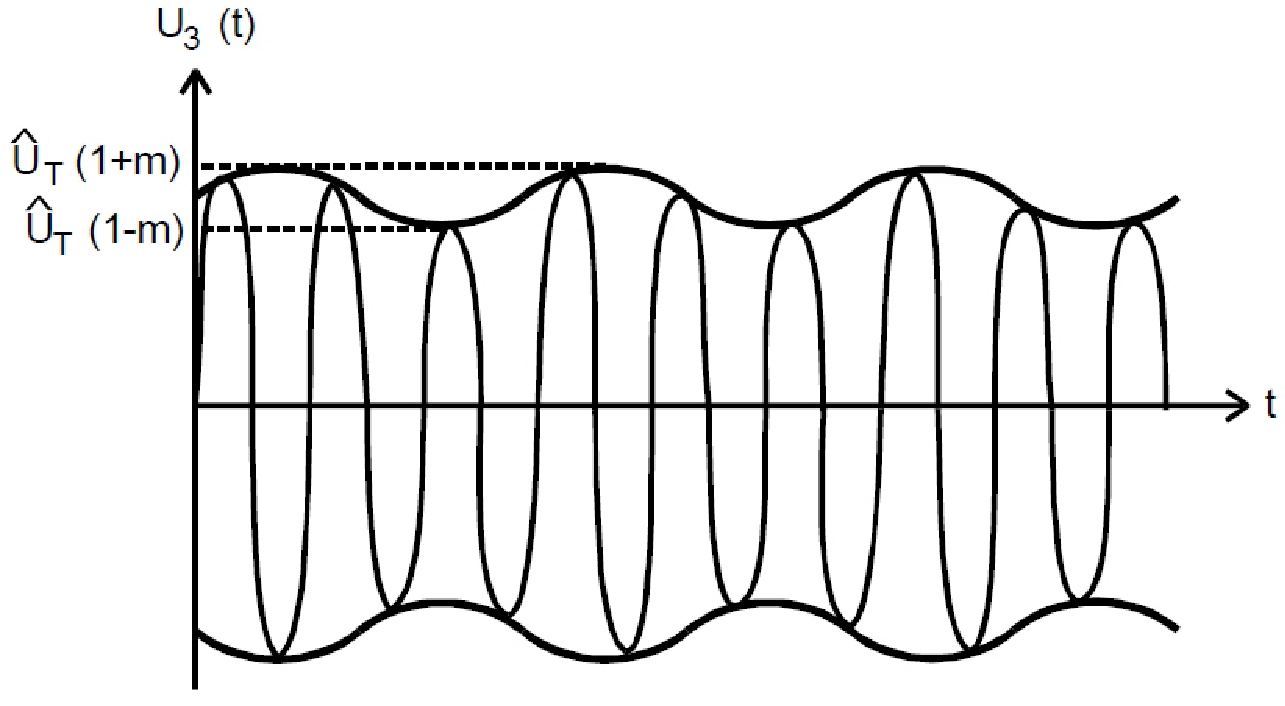
\includegraphics[width = \textwidth]{../Grafiken/Frequenzbaender.pdf}
	\caption{Beispiel für eine Amplitudenmodulierte Spannung.\cite{V59}}
\end{figure}
In einer Schaltung ist eine hochfrequente Trägerspannung $U_T$, die geschrieben werden kann als
\begin{align}
	U_T(t)=\hat U_T\cos\omega_Tt.
\end{align}
Dabei ist $\hat U_T$ die Amplitude und $\omega_T$ die Kreisfrequenz.
Diese wird mithilfe einer Modulationsspannung $U_M$ modelliert, diese wird beschrieben durch
\begin{align}
	U_M(t)=\hat U_M\cos\omega_Mt,
\end{align}
mit der Amplitude $\hat U_M$ und der Kreisfrequenz $\omega_M$.
Die Spannung $U_3$die aus der Modulation entsteht kann geschrieben werden als
\begin{align}
	U_3(t)=\hat U_t\left(1+m\cos\omega_Mt\right)\cos \omega_Tt
\end{align}
mit dem Modulationsgrad $m$, der definiert ist als 
\begin{align}
	m = \gamma \hat U_M
\end{align}
mit der Proportionalitätskonstante $\gamma$ mit der Dimension $\frac{1}{V}$.
Das $m$ liegt zwischen 0 und 1.\\
Die Spannung $U_3$ kann umgeschrieben werden in
\begin{align}
	U_3(t)=\hat U_T\left[\cos\omega_Tt+\frac{1}{2}m\cos\left(\omega_T+\omega_M\right)t+\frac{1}{2}\cos\left(\omega_t-\omega_M\right)t\right]
\end{align}
Daraus lässt sich das Frequenzspektrum ablesen, dieses ist in \cref{fig:Frequenzspektrum} dargestellt.
\begin{figure}
	\centering
	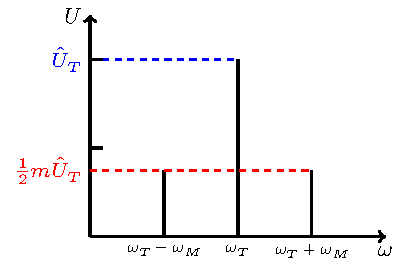
\includegraphics[width =\textwidth/2]{../Grafiken/tikz/tikz-Frequenzspektrum.pdf}
	\caption{Das Frequenzspektrum zu der Amplitudenmodulation.\label{fig:Frequenzspektrum} }
\end{figure}
\newpage
\subsection{Frequenzmodulation}
\begin{figure}[h!]
	\centering
	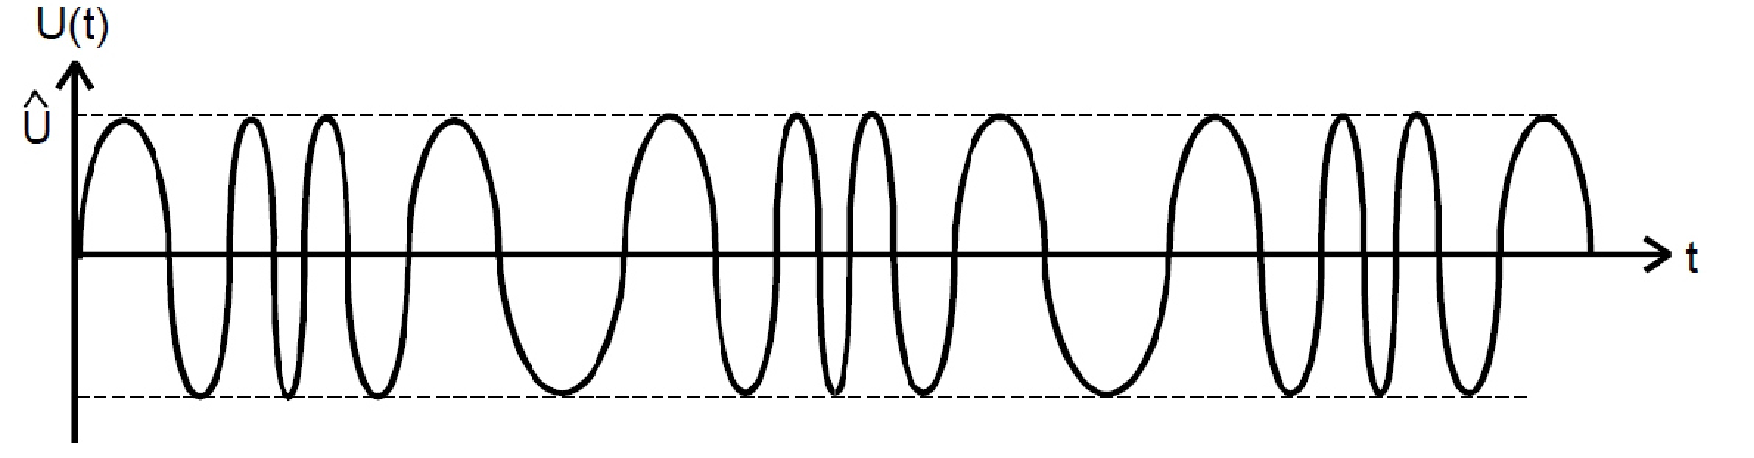
\includegraphics[width = \textwidth]{../Grafiken/Frequenzmodulation.pdf}
	\caption{Darstellung der Änderung einer Frequenzmodulierten Spannung gegen die Zeit.\cite{V59}\label{fig:Frequenzmodulation}}
\end{figure}
Bei der frequenzmodulierten Spannung, ändert sich die Phase beziehungsweise die Frequenz periodisch, wie in \cref{fig:Frequenzmodulation} dargestellt.
Die Spannung einer solcher modulierten Schwingung kann dargestellt werden durch
\begin{align}
	U(t)=\hat U \sin\left(\omega_Tt+m\frac{\omega_T}{\omega_M}\cos\omega_Mt\right)
\end{align}
Daraus lässt sich die momentan Frequenz $f$ bestimmen, durch Ableitung des Arguments vom Sinus.
\begin{align}
	f(t)=\frac{\omega_T}{2\pi}\left(1-m\sin\omega_Mt\right)
\end{align}
Daraus lässt sich der Frequenzhub ablesen als
\begin{align}
	\Delta \omega = m\frac{\omega_T}{2\pi}
\end{align}